% May not get to this in time for Auburn...
\chapter{Gameplay}
\section{Match autos}
Throughout trial and research, we have come to a conclusion that an auto that gets nine to eleven rings in auto is the best for our team, and gives us the best advantage going into driver control.

\subsection{15"}

\subsection{Original}
\begin{itemize}
    \item \subsection{Start}
\end{itemize}
\begin{enumerate}
    \item The robot starts at the coordinate (-2.5, 1.5) for red side, and coordinate (2.5, 1.5) for blue side.
\end{enumerate}
\begin{itemize}
    \item \subsection{Auto}
    \item \subsubsection{Red}
\end{itemize}
\begin{enumerate}
    \item The robot moves to the coordinate (0, 2) with the mobile goal rush are out to grab to mobile goal.
    \item The robot reverses to the coordinate (-1, 1) and releases the mobile goal, and retracts the mobile goal rush arm. 
    \item The robot then turns away from the mobile goal, and reverses to the goal and clamps down.
    \item The robot then moves to the coordinate (-1, 2.5) to intake a red ring, to load onto the mobile goal.
    \item The robot then moves to the coordinate (-2, 2) to intake a red ring, to load onto the mobile goal.
    \item The robot then moves to the coordinate (-2.75, 2.75) and intakes a ring, if red it loads onto the goal if blue it tosses it away.
    \item The robot then reverses to (-2, 2) and then repeats steps six and seven three more times.
    \item The robot then moves to the coordinate (-2.5, 0) on the way releases the mobile goal.
    \item The robot then indexes a red ring, and turns toward negative ninety degrees.
    \item The robot then reverses into the mobile goal at (-2, 0) and clamps down.
    \item The robot intakes to fully score the red ring, then releases the mobile goal.
    \item The robot then moves to (-1, 0) to contact the ladder to get auto win point.
\end{enumerate}
\begin{itemize}
    \item \subsubsection{Blue}
\end{itemize}
\begin{enumerate}
    \item     The robot moves to the coordinate (0, 2) with the mobile goal rush are out to grab to mobile goal.
    \item The robot reverses to the coordinate (1, 1) and releases the mobile goal, and retracts the mobile goal rush arm. 
    \item The robot then turns away from the mobile goal, and reverses to the goal and clamps down.
    \item The robot then moves to the coordinate (1, 2.5) to intake a blue ring, to load onto the mobile goal.
    \item The robot then moves to the coordinate (2, 2) to intake a blue ring, to load onto the mobile goal.
    \item The robot then moves to the coordinate (2.75, 2.75) and intakes a ring, if blue it loads onto the goal if red it tosses it away.
    \item The robot then reverses to (2, 2) and then repeats steps six and seven three more times.
    \item The robot then moves to the coordinate (2.5, 0) on the way releases the mobile goal.
    \item The robot then indexes a blue ring, and turns toward negative ninety degrees.
    \item The robot then reverses into the mobile goal at (2, 0) and clamps down.
    \item The robot intakes to fully score the blue ring, then releases the mobile goal.
    \item The robot then moves to (-1, 0) to contact the ladder to get auto win point.
\end{enumerate}

\subsection{24"}

\subsection{Original}
\begin{itemize}
    \item \subsection{Start}
\end{itemize}
\begin{enumerate}
    \item The robot starts at the coordinate (-1.75, -.5) for red side 1 , and coordinate (1.75, -.5) for blue side 1.
    \item The robot starts at the the coordinate (-1.75, -1.5) for red side 2, and coordinate (1.75, -1.5) for blue side 2.
\end{enumerate}
\begin{itemize}
    \item \subsection{Auto}
    \item \subsubsection{Red 1}
\end{itemize}
\begin{enumerate}
    \item The robot moves to the coordinate (0, 0) and clamps the mobile goal with the mobile goal rush arm.
    \item The robot then reverses to the coordinate (-.5, -.5) and releases the mobile goal.
    \item The robot then turns away from the mobile goal, and reverses into the goal and clamps onto the mobile goal.
    \item The robot then moves to the coordinate (-1, -2) to intake a red ring, to load onto the mobile goal.
    \item The robot then moves to the coordinate (-2, -2) to intake a red ring, to load onto the mobile goal.
    \item The robot then moves to the coordinate (-2.75, -2.75) and intakes a ring, if red it loads onto the goal if blue it tosses it away.
    \item The robot then reverses to (-2, -2) and then repeats steps six and seven, three more times.
    \item The robot then reverses to the coordinate (-2, -2) for the last time and turns away from the corner.
    \item The robot then reverse into the corner and wait until driver.
\end{enumerate}
\begin{itemize}
    \item \subsubsection{Red 2}
\end{itemize}
\begin{enumerate}
    \item The robot moves to the coordinate (0, -2) and clamps the mobile goal with the mobile goal rush arm.
    \item The robot then reverses to the coordinate (-.5, -1.5) and releases the mobile goal.
    \item The robot then turns away from the mobile goal, and reverses into the goal and clamps onto the mobile goal.
    \item The robot then moves to the coordinate (-1, -2) to intake a red ring, to load onto the mobile goal.
    \item The robot then moves to the coordinate (-2, -2) to intake a red ring, to load onto the mobile goal.
    \item The robot then moves to the coordinate (-2.75, -2.75) and intakes a ring, if red it loads onto the goal if blue it tosses it away.
    \item The robot then reverses to (-2, -2) and then repeats steps six and seven three more times.
    \item The robot then reverses to the coordinate (-2, -2) for the last time and turns away from the corner.
    \item The robot then reverse into the corner and wait until driver.
\end{enumerate}
\begin{itemize}
    \item \subsubsection{Blue 1}
\end{itemize}
\begin{enumerate}
    \item The robot moves to the coordinate (0, 0) and clamps the mobile goal with the mobile goal rush arm.
    \item The robot then reverses to the coordinate (.5, -.5) and releases the mobile goal.
    \item The robot then turns away from the mobile goal, and reverses into the goal and clamps onto the mobile goal.
    \item The robot then moves to the coordinate (1, -2) to intake a blue ring, to load onto the mobile goal.
    \item The robot then moves to the coordinate (2, -2) to intake a blue ring, to load onto the mobile goal.
    \item The robot then moves to the coordinate (2.75, -2.75) and intakes a ring, if blue it loads onto the goal if red it tosses it away.
    \item The robot then reverses to (2, -2) and then repeats steps six and seven, three more times.
    \item The robot then reverses to the coordinate (2, -2) for the last time and turns away from the corner.
    \item The robot then reverse into the corner and wait until driver.
\end{enumerate}
\begin{itemize}
    \item \subsubsection{Blue 2}
\end{itemize}
\begin{enumerate}
    \item The robot moves to the coordinate (0, -2) and clamps the mobile goal with the mobile goal rush arm.
    \item The robot then reverses to the coordinate (.5, -1.5) and releases the mobile goal.
    \item The robot then turns away from the mobile goal, and reverses into the goal and clamps onto the mobile goal.
    \item The robot then moves to the coordinate (1, -2) to intake a blue ring, to load onto the mobile goal.
    \item The robot then moves to the coordinate (2, -2) to intake a blue ring, to load onto the mobile goal.
    \item The robot then moves to the coordinate (2.75, -2.75) and intakes a ring, if blue it loads onto the goal if red it tosses it away.
    \item The robot then reverses to (2, -2) and then repeats steps six and seven three more times.
    \item The robot then reverses to the coordinate (2, -2) for the last time and turns away from the corner.
    \item The robot then reverse into the corner and wait until driver.
\end{enumerate}
\subsection{Updated}
After repeated trial, we have come to the conclusion that having match autos for each robot exclusively is not efficient. So we decided to make every auto possible with either bot depending on who were matched up against. So now we have four match autos for each side.
\begin{itemize}
    \item Red\subsubsection{
    \item Negative}
\end{itemize}
\begin{enumerate}
    \item The robot starts at the coordinate (-2.5, 1.25)
    \item The robot then moves to the coordinate (0, 2) and clamp onto the mobile goal with the mobile goal rush arm.
    \item The robot then reverse to the coordinates (-.5, 1.5) and unclamp the mobile goal rush arm, and fold up the mobile goal rush arm.
    \item The robot then turns away from the goal, then backs into the goal and clamps down.
    \item The robot then moves to the coordinate (-1, 2) and intakes a red ring, to score it onto the mobile goal.
    \item The robot then moves to the coordinate (-2, 2) and intakes a red ring, to score it onto the mobile goal.
    \item The robot then moves to the coordinate (2.75, -2.75) and intakes a ring, if blue it loads onto the goal if red it tosses it away.
    \item The robot then reverses to (-2, 2) and then repeats steps seven and eight, three more times.
    \item The robot then reverses to the coordinate (-2, 2) for the last time and turns away from the corner.
    \item The robot then moves to the coordinate (-1, 0) to touch the ladder and get auto win point.
\end{enumerate}
\begin{itemize}
    \item \subsubsection{Negative mid}
\end{itemize}
\begin{enumerate}
    \item The robot starts at the coordinate (-2.5, .75)
    \item The robot then moves to the coordinate (0, 0) and clamp onto the mobile goal with the mobile goal rush arm.
    \item The robot then reverse to the coordinates (-.5, .5) and unclamp the mobile goal rush arm, and fold up the mobile goal rush arm.
    \item The robot then turns away from the goal, then backs into the goal and clamps down.
    \item The robot then moves to the coordinate (-1, 2) and intakes a red ring, to score it onto the mobile goal.
    \item The robot then moves to the coordinate (-2, 2) and intakes a red ring, to score it onto the mobile goal.
    \item The robot then moves to the coordinate (2.75, -2.75) and intakes a ring, if blue it loads onto the goal if red it tosses it away.
    \item The robot then reverses to (-2, 2) and then repeats steps seven and eight, three more times.
    \item The robot then reverses to the coordinate (-2, 2) for the last time and turns away from the corner.
    \item The robot then moves to the coordinate (-1, 0) to touch the ladder and get auto win point.
\end{enumerate}
\begin{itemize}
    \item \subsubsection{Positive mid}
\end{itemize}
\begin{enumerate}
    \item The robot starts at the coordinate (-2.5, -.75)
    \item The robot then moves to the coordinate (0, 0) and clamp onto the mobile goal with the mobile goal rush arm.
    \item The robot then reverse to the coordinates (-.5, -.5) and unclamp the mobile goal rush arm, and fold up the mobile goal rush arm.
    \item The robot then turns away from the goal, then backs into the goal and clamps down.
    \item The robot then moves to the coordinate (-2.5, -.75).
    \item The robot then moves to the coordinate (-2.5, .5) to intake a red ring and load it onto the mobile goal.
    \item The robot releases the mobile goal.
    \item The robot then reverses to the coordinate (-2, 0) to clamp onto a mobile goal.
    \item The robot then goes to the coordinate (-2, .75) and turns toward 180 degrees.
    \item The robot then moves to the coordinate (-1, -2) and intakes a red ring, to score it onto the mobile goal.
    \item The robot then moves to the coordinate (-2, -2) and intakes a red ring, to score it onto the mobile goal.
    \item The robot then moves to the coordinate (-2.75, -2.75) and intakes a ring, if blue it loads onto the goal if red it tosses it away.
    \item The robot then reverses to (-2, 2) and then repeats steps seven and eight, three more times.
    \item The robot then reverses to the coordinate (-2, 2) for the last time and turns away from the corner.
    \item The robot then moves to the coordinate (-1, 0) to touch the ladder and get auto win point.
\end{enumerate}
\begin{itemize}
    \item \subsubsection{Positive}
\end{itemize}
\begin{enumerate}
    \item The robot starts at the coordinate (-2.5, -.75)
    \item The robot then moves to the coordinate (0, 2) and clamp onto the mobile goal with the mobile goal rush arm.
    \item The robot then reverse to the coordinates (-.5, -1.5) and unclamp the mobile goal rush arm, and fold up the mobile goal rush arm.
    \item The robot then turns away from the goal, then backs into the goal and clamps down.
    \item The robot then moves to the coordinate (-2.5, -.75).
    \item The robot then moves to the coordinate (-2.5, .5) to intake a red ring and load it onto the mobile goal.
    \item The robot releases the mobile goal.
    \item The robot then reverses to the coordinate (-2, 0) to clamp onto a mobile goal.
    \item The robot then goes to the coordinate (-2, .75) and turns toward 180 degrees.
    \item The robot then moves to the coordinate (-1, -2) and intakes a red ring, to score it onto the mobile goal.
    \item The robot then moves to the coordinate (-2, -2) and intakes a red ring, to score it onto the mobile goal.
    \item The robot then moves to the coordinate (-2.75, -2.75) and intakes a ring, if blue it loads onto the goal if red it tosses it away.
    \item The robot then reverses to (-2, 2) and then repeats steps seven and eight, three more times.
    \item The robot then reverses to the coordinate (-2, 2) for the last time and turns away from the corner.
    \item The robot then moves to the coordinate (-1, 0) to touch the ladder and get auto win point.
\end{enumerate}
\begin{figure}
    \centering
    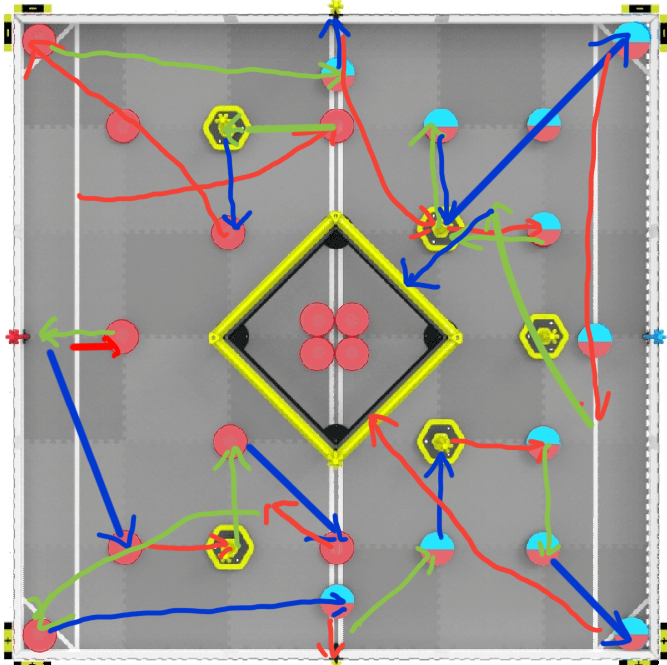
\includegraphics[width=0.5\linewidth]{images/misc/Auto-Map.jpg}
    \caption{Auto map for skills}
    \label{fig:Auto map}
\end{figure}

\section{Skills}
The goal is to score at least a combined 62 point auto skills. we achieve this goal by filling four mobile goals with four red rings each. Then place the four mobile goals in the corners. In addition, we place one red ring on the fifth mobile goal. We also place one red ring on each of the neutral wall stakes, and one red on the red alliance wall stake. After scoring all of the rings we desire, both of the robots go for a tier one hang. \ref{fig:Auto map}.

\subsection{15"}
\begin{itemize}
    \item \subsubsection{Start}
\end{itemize}
\begin{enumerate}
    \item The 15" robot starts at the coordinate (-2.5, 1.5).
\end{enumerate}
\begin{itemize}
    \item \subsubsection{First mobile goal}
\end{itemize}
\begin{enumerate}
    \item The robot moves to the coordinate (.25, 2) to index a red ring.
    \item The robot then backs up to the coordinate (-1.25, 2) and then clamp down onto the mobile goal.
    \item The robot then intakes to fully load the red ring in the intake onto the mobile goal to be the first ring loaded.
    \item The robot the moves to the coordinate (-1, 1) to intake a red ring, to load the second red ring onto the mobile goal.
    \item The robot then moves to the coordinate (-2, 2) to intake a red ring, to load the third red ring onto the mobile goal.
    \item The robot then moves to the coordinate (-2.75, 2.75) to intake a red ring, to load the fourth ring onto the mobile goal.
    \item The robot then backs up to the coordinate (-2, 2) to turn away from the corner.
    \item The robot then backs up to the coordinate (-2.75, 2.75) to unclamp and drop off the mobile goal into the corner.
\end{enumerate}
\begin{itemize}
    \item \subsubsection{Lady brown}
\end{itemize}
\begin{enumerate}
    \item The robot moves forward to the coordinate (-2, 2) and then turn toward one hundred degrees.
    \item The robot then moves to the coordinate (.5, 2.5) to load a red ring into the lady brown.
    \item The robot then backs up to the coordinate (0, 2) to line up with the neutral wall stake.
    \item The robot then moves to the coordinate (0, 3) to move up to the neutral wall stake.
    \item The lady brown then fully extends and places the red ring onto the neutral wall stake.
\end{enumerate}
\begin{itemize}
    \item \subsubsection{Second mobile goal}
\end{itemize}
\begin{enumerate}
    \item The robot reverses to the coordinate (0, 2) and the lady brown comes to a rest.
    \item The robot then reverses to the coordinate (1, 1) to then clamp onto the mobile goal. 
    \item The robot then moves to the coordinate (1, 2) to intake a red ring, to load the first onto the mobile goal.
    \item The robot then moves to the coordinate (2, 1) to intake a red ring, to load the second ring onto the mobile goal.
    \item The robot then moves to the coordinate (2, 2) to intake a red ring, to load the third ring onto the mobile goal.
    \item The robot then moves to the coordinate (2.75, 2.75) to intake a red ring, to load the fourth ring onto the mobile goal.
    \item The robot then reverses to the coordinate (2, 2).
    \item The robot then moves to the coordinate (2.75, 2.75) to intake a blue ring, to remove the blue ring from the corner.
    \item The robot then reverses to the coordinate (2, 2).
    \item The robot then turns away from the corner and reverses to the coordinate (2.75, 2.75) to drop off the mobile goal.
\end{enumerate}
\begin{itemize}
    \item \subsubsection{Third mobile goal}
\end{itemize}
\begin{enumerate}
    \item The robot moves forward to the coordinate (2.5, 2.5).
    \item The robot the moves to the coordinate (2.5, -.75) to index a red ring.
    \item The robot then turns away from the coordinate (2, 0).
    \item The robot then reverses to the coordinate (1.75, .25) and then clamp onto the mobile goal.
    \item The robot then intakes to fully load the red ring onto the mobile goal.
\end{enumerate}
\begin{itemize}
    \item \subsubsection{Hang}
\end{itemize}
\begin{enumerate}
    \item The robot release the mobile goal and then moves to the coordinate (2, 2).
    \item The robot then turns towards forty five degrees.
    \item the robot then fully extends the lady brown and mobile goal rush arm, as the robot moves toward the coordinate (.5, .5).
    \item Lastly the robot reverses into its final hanging position.
\end{enumerate}

\subsection{24"}
    \begin{itemize}
        \item \subsubsection{Start}
    \end{itemize}
    \begin{enumerate}
        \item The 24" robot starts at the coordinates (-2.5, 0).
    \end{enumerate}
\begin{itemize}
    \item Red alliance wall stake
\end{itemize}
        \begin{enumerate}
            \item The robot then moves to coordinates (-2, 0) to grab the red ring in front of the robot, then returns to the starting position to intake the red ring onto the red alliance wall stake.
        \end{enumerate}
    \begin{itemize}
        \item \subsubsection{First mobile goal}
    \end{itemize}
    \begin{enumerate}
        \item The robot moves to the coordinate (-2, -2) to index a red ring.
        \item The robot then reverses into the mobile goal at the coordinate (-1, -2) and clamp onto the mobile goal.
        \item  The robot then fully intakes the red ring previously indexed, to start filling the mobile goal.  
        \item The robot then moves tot the coordinate (-1, -1) to intake a red ring, to load the second ring onto the mobile goal.
        \item The robot then moves to the coordinate (0, -2) to intake a red ring, to load the third ring onto the mobile goal.
        \item The robot then moves to the coordinate (-2, -2) to prepare to get the corner at the coordinate (-3, -3).
        \item   The robot then moves to the coordinate (-2.75, -2.75) to intake a red ring, to load the fourth ring onto the mobile goal.
        \item   The robot then reverses to the coordinate (-2, -2) then turns away from the corner.
        \item   The robot then reverse to the coordinates (-2.75, -2.75) to then release the mobile goal in the corner.
    \end{enumerate}
   \begin{itemize}
       \item \subsubsection{Lady brown}
   \end{itemize}
\begin{enumerate}
    \item The robot then moves to the coordinates (-2, -2) and turn toward ninety degrees to prepare for the lady brown.
    \item  The robot then moves to the coordinate (.25, -2.5) to grab the red ring and load into the lady brown. 
    \item The robot then reverses to the coordinate (0, -2) to line up for the lady brown.
    \item   The robot then moves to the coordinate (0, -3) to go up to the neutral wall stake, and then extend the lady brown arm fully to place the red ring on the neutral wall stake. 
\end{enumerate}
\begin{itemize}
    \item \subsubsection{Second mobile goal}
\end{itemize}
\begin{enumerate}
    \item The robot then reverses to the coordinate (0, -2).
    \item The robot moves to the coordinate (1, -2) to index a red ring. 
    \item The robot then reverses to the coordinate (1, -1) to clamp onto the mobile goal, and then intakes the red ring all the way onto the mobile goal, to be the first ring on the goal.
    \item The robot then moves to the coordinate (2, -1) to intake a red ring, to put the second on the mobile goal.
    \item The robot then moves to the coordinate (2, -2) to intake a red ring, to put the third ring onto the mobile goal. 
    \item The robot then moves to the coordinate (2.75, -2.75) to then intake a red ring in the corner, to load the fourth onto the mobile goal.
    \item The robot then reverses to the coordinate (2, -2).
    \item The robot then moves to the coordinate (2.75, -2.75) again to intake a blue ring, to remove it from the corner.
    \item The robot then moves to the coordinate (2, -2) and turn away from the corner at the coordinates (3, -3). 
    \item   The robot then reverses into corner at the coordinate (3, -3) and release the clamp.
\end{enumerate}
\begin{itemize}
    \item \subsubsection{Hang}
\end{itemize}
\begin{enumerate}
    \item The robot then moves to the coordinate (2, -2) and turn toward the corner at the coordinates (3, -3).
    \item The robot then fully extends the lady brown and the mobile goal rush arm to prepare for hang.
    \item  The robot moves toward the coordinate (.5, -.5).
    \item  Lastly the robot reverses to fully hang the robot.
\end{enumerate}